\documentclass[12pt,t]{beamer}

\usetheme{default}
\beamertemplatenavigationsymbolsempty
\hypersetup{pdfpagemode=UseNone} % don't show bookmarks on initial view

\definecolor{background}{RGB}{255,255,255}
\definecolor{foreground}{RGB}{24,24,24}
\definecolor{title}{RGB}{107,174,214}
\definecolor{gray}{RGB}{155,155,155}
\definecolor{darkBlue}{RGB}{27,84,124}
\definecolor{darkGray}{RGB}{75,75,75}
\definecolor{subtitle}{RGB}{102,255,204}
\definecolor{hilight}{RGB}{102,255,204}
\definecolor{vhilight}{RGB}{255,111,207}

\setbeamercolor{titlelike}{fg=title}
\setbeamercolor{subtitle}{fg=subtitle}
\setbeamercolor{institute}{fg=gray}
\setbeamercolor{normal text}{fg=foreground,bg=background}

\setbeamercolor{item}{fg=foreground} % color of bullets
\setbeamercolor{subitem}{fg=gray}
\setbeamercolor{itemize/enumerate subbody}{fg=gray}
\setbeamertemplate{itemize subitem}{{\textendash}}
\setbeamerfont{itemize/enumerate subbody}{size=\footnotesize}
\setbeamerfont{itemize/enumerate subitem}{size=\footnotesize}

%\setbeamertemplate{footline}{%
%    \raisebox{5pt}{\makebox[\paperwidth]{\hfill\makebox[20pt]{\color{gray}
%          \scriptsize\insertframenumber}}}\hspace*{5pt}}



\usepackage[utf8]{inputenc}
\usepackage[english]{babel}
\usepackage[T1]{fontenc}

\usepackage{multicol}
\usepackage{booktabs}
\usepackage{tikz}
\usepackage[ruled,vlined,english]{algorithm2e}
\usetikzlibrary{arrows,automata,shapes,positioning,calc}

\usepackage{float} % placement des figures
\usepackage{amssymb} % symboles mathématiques
\usepackage{graphicx} % affichage d'images
\usepackage{url} % inclure des urls



\title{GitHub activity}
\subtitle{}
\date{January 23, 2015}
\institute{École Normale Supérieure de Lyon}
\author{Quentin Cormier, Tom Cornebize, Yassine Hamoudi}

\begin{document}

\maketitle

\begin{frame}
    \frametitle{GitHub?}
    \begin{columns}
    \begin{column}{0.4\textwidth}
        \vspace{1cm}
        \begin{figure}
        
\includegraphics[width=0.9\textwidth]{Octocat.png}
        \end{figure}
    \end{column}
    \begin{column}{0.6\textwidth}
        \vspace{2cm}
        \begin{itemize}
            \item A web-based Git repository hosting service
            \item More than 3 million users
            \item More than 10 million repositories
        \end{itemize}
    \end{column}
    \end{columns}
\end{frame}

\begin{frame} % Events on 48h the 1 and 2 January 2015
    \frametitle{Type of events}
    % From http://www.texample.net/tikz/examples/pie-chart-color/
    \def\angle{0}
    \def\radius{3}
    \def\cyclelist{{"title","gray","title","gray"}}
    \newcount\cyclecount \cyclecount=-1
    \newcount\ind \ind=-1
    \begin{figure}
    \resizebox{.9\linewidth}{!}{
    \begin{tikzpicture}[nodes = {font=\sffamily}]
      \foreach \percent/\name in {
        52.1/PushEvent,
        10.9/CreateEvent,
        10.0/WatchEvent,
        9.1/IssueCommentEvent,
        5.0/IssuesEvent,
        4.3/PullRequestEvent,
        3.2/ForkEvent,
        5.4/Other events
%        1.7/DeleteEvent,
%        1.3/PullRequestReviewCommentEvent,
%        1.0/GollumEvent,
%        0.6/CommitCommentEvent,
%        0.4/ReleaseEvent,
%        0.3/MemberEvent,
%        0.1/PublicEvent
        } {
          \ifx\percent\empty\else               % If \percent is empty, do nothing
            \global\advance\cyclecount by 1     % Advance cyclecount
            \global\advance\ind by 1            % Advance list index
            \ifnum3<\cyclecount                 % If cyclecount is larger than list
              \global\cyclecount=0              %   reset cyclecount and
              \global\ind=0                     %   reset list index
            \fi
            \pgfmathparse{\cyclelist[\the\ind]} % Get color from cycle list
            \edef\color{\pgfmathresult}         %   and store as \color
            % Draw angle and set labels
            \draw[fill={\color!50},draw={\color}] (0,0) -- (\angle:\radius)
              arc (\angle:\angle+\percent*3.6:\radius) -- cycle;
            \node at (\angle+0.5*\percent*3.6:0.7*\radius) {\percent\,\%};
            \node[pin=\angle+0.5*\percent*3.6:\name]
              at (\angle+0.5*\percent*3.6:\radius) {};
            \pgfmathparse{\angle+\percent*3.6}  % Advance angle
            \xdef\angle{\pgfmathresult}         %   and store in \angle
          \fi
        };
    \end{tikzpicture}
    }
    \end{figure}
\end{frame}

\begin{frame}
    \frametitle{One week activity}
        Number of commits per day.
        Max at 15h20 UTC.
        \begin{figure}
        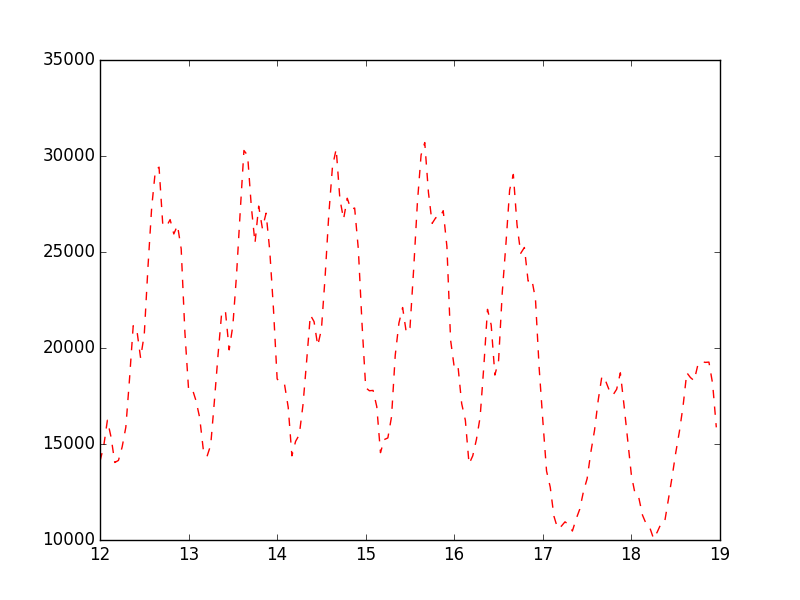
\includegraphics[width=0.9\textwidth]{oneweekofactivity.png}
        \end{figure}
\end{frame}

\begin{frame}
    \frametitle{Conclusion}
    
    Use our scripts:
    \begin{center}
      https://github.com/robocop/GithubAnalysis
    \end{center}
   
    \begin{center}
        
\includegraphics[width=0.2\textwidth]{octocat2.png}
    \end{center}

    Download the data:
    \begin{center}
      https://www.githubarchive.org/
    \end{center}

\end{frame}


\end{document}
